\documentclass[aspectratio=169,11pt]{beamer}
\usetheme{default}
\usecolortheme{whale}
\setbeamertemplate{navigation symbols}{}
\setbeamertemplate{footline}{%
  \hbox{\begin{beamercolorbox}[wd=\paperwidth,ht=2.2ex,dp=1ex,leftskip=1.2em,rightskip=1.2em]{author in head/foot}%
    \tiny\itshape S4D: state-of-the-art hierarchical speculative decoding\hfill\upshape\insertframenumber\,/\,\inserttotalframenumber%
  \end{beamercolorbox}}%
}
\setbeamerfont{frametitle}{series=\bfseries}
\setbeamercolor{frametitle}{fg=white,bg=structure}
\usepackage{graphicx}
\usepackage{tikz}
\usetikzlibrary{arrows.meta,positioning}
\usepackage{amsmath}
\usepackage{booktabs}
\usepackage{colortbl}
\setbeamertemplate{itemize items}[circle]
\setbeamertemplate{note page}{\insertnote}

% ---- toggle notes: `\setbeameroption{show notes}` for the notes build ----

\title{\textbf{Self-Taught Semi-Self Speculative Decoding}}
\subtitle{\textbf{S4D}: a learned routing policy that \textbf{Pareto-dominates} hierarchical speculative decoding}
\author{viasd-rl}
\date{\today}

\begin{document}

\begin{frame}\titlepage
\vspace{-3mm}
\begin{center}\small
\textbf{The new state of the art in hierarchical speculative decoding.}\\[2pt]
A strict Pareto improvement: up to \textbf{$3.5\times$ faster}, while \emph{preserving} accuracy (lossless quality at \textbf{$4\times$ fewer} model calls).
\end{center}
\end{frame}
\note{
Hi everyone. Our project is S4D, which stands for Self-Taught Semi-Self Speculative Decoding. The
name actually encodes the whole method, and I'll unpack each piece as we go. ``Speculative Decoding''
is the base technique that makes language models faster. ``Semi-Self'' is the clever part of the
method we build on: the model verifies its own draft using a reduced copy of itself. And ``Self-Taught''
is our contribution: instead of hand-tuning the decision rule, the model learns its own routing policy
with reinforcement learning. The result wins: it matches lossless quality at a fraction of the cost,
and beats the hand-tuned baseline across the board. Let me show you.
}

% =====================================================================
\begin{frame}{Overview}
\textbf{We introduce the first reinforcement-learned routing policy for hierarchical speculative decoding, and set a new state of the art.}
\vspace{6pt}

{\footnotesize VIA-SD adds a slim intermediate verifier, but routes between tiers using confidence thresholds tuned by hand.}
\vspace{4pt}

We present \textbf{three key contributions}:
\begin{enumerate}
  \item A \textbf{learned per-token gating policy} that recasts tier-routing as a sequential decision problem, so a tiny $q$-free MLP replaces the fixed thresholds.
  \item A \textbf{reward} that balances output quality against the latency of expensive verifier calls.
  \item A \textbf{per-token RL formulation} with principled credit assignment (REINFORCE, then GRPO, then a per-token advantage).
\end{enumerate}
\vspace{2pt}
{\footnotesize\textbf{The payoff:} we match \emph{lossless} accuracy (\textbf{0.91}) at \textbf{4$\times$ fewer} full-model calls,
\textbf{2.2$\times$} faster than greedy. We \textbf{Pareto-dominate} the paper's VIA-SD at roughly \textbf{2$\times$ its speedup and 2.3$\times$ its accuracy},
and reach up to \textbf{3.5$\times$} when pushed for speed.}
\end{frame}
\note{
Here is the whole project on one slide. We built the first \emph{learned} router for hierarchical
speculative decoding. There are three contributions, and I'll give one slide to each. One: a learned
per-token gate, a tiny network that decides, token by token, how much compute to spend. Two: a reward
that balances output quality against cost. Three: a per-token reinforcement-learning setup that
actually trains it well. And the payoff, which I'll keep coming back to: we match lossless accuracy,
0.91, at four times fewer expensive model calls. We Pareto-dominate VIA-SD, at roughly twice its
speedup and over twice its accuracy. And pushed for speed, we go up to three and a half times faster.
Let me unpack it.
}

% =====================================================================
\begin{frame}{The bottleneck: LLM decoding is slow and sequential}
\begin{itemize}
  \item Generating each token streams the entire model from memory, so LLM inference is memory-bandwidth bound and dominated by sequential forward passes.
  \item Speculative decoding fixes this: a cheap \emph{drafter} guesses several tokens, and the big \emph{verifier} checks them all in one parallel pass.
  \item Accepted guesses give many tokens per expensive forward. It is \textbf{lossless}, and runs about \textbf{1.4$\times$} faster (wall-clock) on our models.
  \item The one lever is the \textbf{acceptance rate}, because every rejected token forces a full-model step.
\end{itemize}
\end{frame}
\note{
First, why speed matters at all. Generating a single token from a big model means reading every one
of its weights out of memory. It's sequential, and it's the dominant cost of LLM inference, both
latency and dollars. Speculative decoding is the standard fix. A small, cheap model guesses the next
few tokens. The big model then checks all of those guesses in a single parallel pass. When the
guesses are right, you got several tokens for the price of one big step, and the output is provably
identical to normal decoding, so it's free quality-wise. On our models that's about 1.4 times faster.
And the one thing that controls the whole method is the acceptance rate: every wrong guess wastes the
speculation and forces a full, expensive step.
}

% =====================================================================
\begin{frame}{VIA-SD improves on vanilla SD}
\begin{columns}
\begin{column}{0.56\textwidth}
Vanilla SD makes a \textbf{binary} choice per token: accept the drafter, or reject and pay for the full model $q$.
\vspace{5pt}

VIA-SD adds a \textbf{slim middle verifier $q'$} (the target $q$ with about 45\% of its layers skipped), giving \textbf{three} choices.
Borderline ``middle-zone'' tokens are handled cheaply by $q'$, so the full model is called far less often.
\vspace{4pt}

{\footnotesize Since $q'$ is the target verifying its \emph{own} draft through a reduced copy of itself, this is the \textbf{Semi-Self} in S4D.}
\end{column}
\begin{column}{0.44\textwidth}
\centering
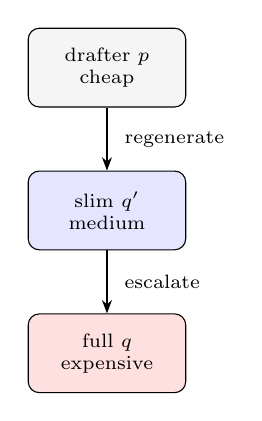
\begin{tikzpicture}[font=\scriptsize,>=Stealth,
  m/.style={draw,rounded corners,minimum width=20mm,minimum height=10mm,align=center}]
\node[m,fill=gray!8] (p) {drafter $p$\\\scriptsize cheap};
\node[m,below=8mm of p,fill=blue!10] (qp) {slim $q'$\\\scriptsize medium};
\node[m,below=8mm of qp,fill=red!12] (q) {full $q$\\\scriptsize expensive};
\draw[->](p)--(qp) node[midway,right=1mm]{regenerate};
\draw[->](qp)--(q) node[midway,right=1mm]{escalate};
\end{tikzpicture}
\end{column}
\end{columns}
\end{frame}
\note{
Now, vanilla speculative decoding is all-or-nothing: you either accept the small model's guess, or
you reject it and pay full price for the big model. VIA-SD's insight is that a lot of those rejected
tokens are borderline. The draft was almost right, it just wasn't certain. So VIA-SD adds a middle
option: the same big model, but with about 45 percent of its layers skipped. It's cheaper than the
full model but still much smarter than the drafter. Now every token has three choices: accept the
draft, regenerate it with this slim middle model, or escalate all the way to the full model.
Borderline tokens get handled by the cheap middle tier, so you call the expensive full model far less
often. And note: because q-prime is just the target verifying its own draft through a reduced copy of
itself, this is the ``Semi-Self'' in our name. It's a genuinely good idea. But it raises one question:
how does it decide which of the three tiers to use?
}

% =====================================================================
\begin{frame}{But it routes with thresholds that are picked by hand}
VIA-SD makes the three-way choice with \textbf{two fixed confidence thresholds} on $q'$:
\quad $\boxed{\alpha_1 = 0.5}$ \quad $\boxed{\alpha_2 = 0.3}$.
\vspace{4pt}
\begin{itemize}
  \item They are \textbf{global and static}: one cutoff for every token and every context.
  \item They are \textbf{brittle}, and must be re-tuned for each new model and task.
  \item They are \textbf{sub-optimal}: even after a full sweep, accuracy peaks at $0.50$ on our setup.
\end{itemize}
\vspace{4pt}
Choosing a tier for each token, from its context, is a sequential decision problem. \textbf{So we learn it} --- the gate teaches itself. That is the \textbf{Self-Taught} in S4D.
\end{frame}
\note{
And here is the catch, the reason the whole project exists. VIA-SD makes that three-way decision with
two numbers picked by hand: zero-point-five and zero-point-three. They're confidence thresholds. And
they have three problems. They're global and static, the same cutoff for every token regardless of
context. They're brittle, so you have to re-tune them for every new model and every new task. And
they're simply sub-optimal: when we swept all nine threshold configurations, accuracy still capped at
0.50 on our setup. The mechanism, which I'll detail at the results, is that the slim verifier is
miscalibrated, so a single global confidence cutoff cannot separate confident-and-correct tokens from
confident-but-wrong ones, and the wrong ones it accepts compound into wrong answers. But step back.
Deciding how much compute to spend on each token, based on that
token's context, is a textbook sequential decision problem. So instead of hand-picking two numbers,
the gate teaches itself the policy. That is the ``Self-Taught'' in S4D, and it gives us our three contributions.
}

% =====================================================================
\section{Method}
\begin{frame}{Contribution 1/3: a learned per-token gating policy (MDP)}
\begin{columns}
\begin{column}{0.56\textwidth}
\small We recast tier-routing as a \textbf{Markov decision process}:
\begin{itemize}
  \item \textbf{State} $s_t$: $q$-free features (drafter/$q'$ confidence, agreement, $\mathrm{KL}(p\Vert q')$, position).
  \item \textbf{Action} $a_t\in\{$accept, regenerate, escalate$\}$.
  \item \textbf{Policy} $\pi_\theta(a_t\mid s_t)$: a tiny MLP.
\end{itemize}
\vspace{3pt}
\footnotesize The full model $q$ is consulted only to \emph{score} at train time. It is never a gate input,
so the gate is free to run at inference.
\end{column}
\begin{column}{0.44\textwidth}
\centering
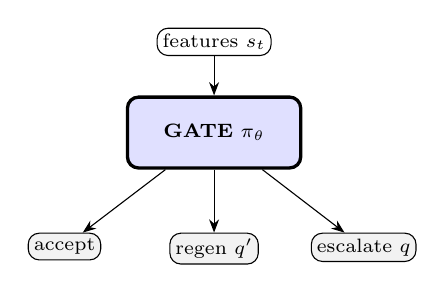
\begin{tikzpicture}[font=\scriptsize,>=Stealth,
  g/.style={draw,very thick,fill=blue!12,rounded corners,minimum width=22mm,minimum height=9mm,align=center},
  a/.style={draw,rounded corners,fill=gray!10,align=center,inner sep=2pt},
  io/.style={draw,rounded corners,align=center,inner sep=2pt}]
\node[io] (f) {features $s_t$};
\node[g,below=5mm of f] (g) {\textbf{GATE} $\pi_\theta$};
\node[a,below=8mm of g,xshift=-19mm] (x){accept};
\node[a,below=8mm of g] (y){regen $q'$};
\node[a,below=8mm of g,xshift=19mm] (z){escalate $q$};
\draw[->](f)--(g);\draw[->](g)--(x);\draw[->](g)--(y);\draw[->](g)--(z);
\end{tikzpicture}
\end{column}
\end{columns}
\end{frame}
\note{
Contribution one: the learned gate. We frame routing as a Markov decision process. The state, for each
token, is a handful of cheap features: how confident the drafter and the slim model are, whether they
agree, how far apart their distributions are, and where we are in the block. The action is which of
the three tiers to use. And the policy is a tiny MLP. The single most important design choice is on
the right of this slide: the features never include the full model. We only ever run the full model
to compute rewards during training. So at inference time, the gate makes its decision instantly, from
cheap signals, without running the expensive model just to decide. That's what makes it free to
deploy: there's no second large model in the serving path.
}

% =====================================================================
\begin{frame}{Contribution 2/3: a reward balancing quality and cost}
\textbf{Two ingredients per token:}
\begin{align*}
\text{quality:}\quad & \text{match}_t = \mathbf{1}\big[\hat y_t = \arg\max\nolimits_v q(v\mid x_{<t})\big] \\[-1pt]
\text{cost:}\quad & \text{cost}_t = \big(t_{p_1} + t_{q'}/\gamma + \mathbf{1}[\textsc{escalate}]\,t_q\big)\big/\,t_{q_1}
\end{align*}
\textbf{Reward} (cost in units of one full-model step):
\begin{align*}
\text{trajectory:}\ & R = \overline{\text{match}} - \lambda\,\overline{\text{cost}}\ (+\,r_c\,\text{correct})
\qquad\qquad
\text{per-token:}\ r_t = \text{match}_t - \lambda\,\text{cost}_t
\end{align*}
\centering\footnotesize $\lambda$ is the quality-versus-speed knob. \texttt{match} is a \emph{dense} proxy for the
sparse true objective (final-answer correctness).
\end{frame}
\note{
Contribution two: the reward, and this is where we pull from the writeup directly. There are two
ingredients per token. Quality is simple: does the token we actually emit match the token the full
model would have produced? That's the match term, and we compute it by running the full model at
training time only. Cost is the per-action latency: the drafter step, plus the slim model amortized
over the block, plus the full model, but only if we escalate, all normalized by the cost of one
full-model step. The reward is just match minus lambda times cost. Lambda is the knob that trades
accuracy for speed. Now the one honest subtlety, and we measured it: matching the full model token by
token is only a proxy for what we truly care about, which is getting the final answer right. They are
not the same thing. Ninety-eight and a half percent token match still left us at only 0.72 final
accuracy, because a couple of slips can derail a whole chain of reasoning. That tension drives a lot
of our analysis.
}

% =====================================================================
\begin{frame}{Contribution 3/3: per-token RL with credit assignment}
\textbf{Policy gradient} (all variants, plus an entropy bonus $\eta\,\mathcal{H}[\pi_\theta]$):
\[
\nabla_\theta J = \mathbb{E}\Big[\textstyle\sum_t A_t\,\nabla_\theta \log \pi_\theta(a_t\mid s_t)\Big]
\]
They differ only in the \textbf{advantage} $A_t$:
\begin{itemize}\small
  \item \textbf{REINFORCE} (trajectory): $A = R - b$, with EMA baseline $b\leftarrow(1{-}\tau)b+\tau R$.
  \item \textbf{GRPO} (group): $A_i = \dfrac{R_i-\mathrm{mean}_{\mathcal G}R}{\mathrm{std}_{\mathcal G}R}$, with PPO-clip $\rho_t=\frac{\pi_\theta}{\pi_{\theta_{\text{old}}}}$ and KL to $\pi_{\text{ref}}$.
  \item \textbf{per-token (v2):} $\hat A_t = \dfrac{r_t-\mathrm{mean}_{\text{batch}}\,r}{\mathrm{std}_{\text{batch}}\,r}$, local credit and the \textbf{lowest variance}.
\end{itemize}
\end{frame}
\note{
Contribution three: how we actually optimize the gate. All three methods share the same skeleton, a
policy gradient. In words: increase the probability of actions that did better than a baseline, and
add an entropy bonus so it keeps exploring. The methods differ in exactly one thing: how they compute
that ``did better than baseline'' term, the advantage. REINFORCE takes one reward for the whole
sequence, subtracts a running average, and applies it to every decision. Simple, but very noisy.
GRPO runs several rollouts of the same prompt and scores each against the group, which cancels out
how hard the prompt is, and it's the right tool for sparse rewards; it also adds PPO clipping and a KL
leash to the starting policy for stability. Our per-token version gives every single decision its own
advantage. Because routing is fundamentally a local choice, this is the lowest-variance signal and it
trains best. The one-line lesson: credit assignment is the whole game here.
}

% =====================================================================
\section{Results}
\begin{frame}{Training converges, and per-token (v2) is cleanest}
\centering

\includegraphics[width=0.9\textwidth]{results/figures/rl_curves.png}
\end{frame}
\note{
Quick proof that the training works. All three methods converge: reward climbs, agreement with the
full model rises to about 0.95, and the rejection rate falls. The interesting part is the variance.
GRPO, in orange, is jumpy, because it only gets one signal per group. REINFORCE, in green, is in the
middle. And our per-token method, in blue, is the smoothest and drives rejections the lowest, exactly
because every decision gets its own credit instead of sharing one reward across the whole sequence.
One detail worth flagging: match plateaus around 0.95, not 1.0, because the q-free features can't
perfectly flag every token the drafter will get wrong. That five-percent residual mismatch is exactly
what compounds into the accuracy gap we discuss later. This is the evidence for the credit-assignment
claim on the last slide.
}

% =====================================================================
\begin{frame}{Results: the learned gate dominates}
\centering\small
\begin{tabular}{lccc}
\toprule
Method & GSM8K acc & q-calls/tok & speedup \\
\midrule
greedy-$q$ (reference)        & 0.887 & 1.000 & 1.00$\times$ \\
plain SD (standard, lossless) & 0.907 & 0.259 & 1.40$\times$\textsuperscript{\dag} \\
\midrule
\rowcolor{red!8} via\_fixed (paper, tuned)  & 0.40 & 0.31 & 1.76$\times$ \\
\rowcolor{red!8} via\_imit (imitation only) & 0.34 & 0.29 & 1.69$\times$ \\
\midrule
\rowcolor{blue!8} via\_rl REINFORCE          & 0.880 & 0.243 & 2.29$\times$ \\
\rowcolor{blue!8} via\_rl GRPO               & 0.853 & \textbf{0.162} & 2.94$\times$ \\
\rowcolor{blue!8} via\_rl REINFORCE+DIMR     & \textbf{0.907} & 0.250 & 2.22$\times$ \\
\rowcolor{blue!8} via\_rl v2 per-token       & 0.713 & 0.104 & \textbf{3.53$\times$} \\
\bottomrule
\end{tabular}
\vspace{2pt}
{\footnotesize \textsuperscript{\dag}wall-clock; via\_* speedups are the overhead-free bandwidth model (not directly comparable).}\\[2pt]
\centering\structure{\textbf{$\Rightarrow$ S4D is state-of-the-art hierarchical speculative decoding.}}
\end{frame}
\note{
Here are the numbers, and I'll give the mechanism behind each row, not just the values. The top two
are references: greedy decoding and lossless speculative decoding. They should be identical, because
speculative decoding is exact; the tiny gap, 0.887 versus 0.907, is just bf16 numerical noise flipping
a couple of borderline problems. Now the red rows, the hand-tuned thresholds, at 0.34 and 0.40. Here
is why they're so low, and this is the key mechanistic point. The threshold accepts a token whenever a
confidence score clears a fixed cutoff. But q-prime is a degraded model with about half its layers
skipped, so its confidence is miscalibrated: it is frequently confident and wrong. A single global
cutoff cannot separate confident-and-correct from confident-but-wrong, so it waves through a stream of
locally-plausible but globally-wrong tokens. And on GSM8K the final answer is all-or-nothing, so even a
two-or-three-percent per-token error rate compounds over a hundred-plus tokens into a wrong answer.
That is also why a full nine-config sweep still caps at 0.50: there is no single cutoff that is right
in every context. The imitation-only baseline is even worse, 0.34, because imitation learning adds exposure bias: it was
trained on near-greedy states but drifts at its own states and over-accepts even more. The blue rows
fix exactly this. RL trains on the policy's own rollouts, which kills the exposure bias, and the match
reward teaches the gate to escalate precisely on the tokens where the drafter would err.
REINFORCE-plus-DIMR recovers full accuracy, 0.907, matching lossless, because a better q-prime makes
the middle tier trustworthy enough to reproduce the full model's output. GRPO drives the expensive-call
count to the floor, 0.16 per token. And the per-token version trades accuracy down to 0.71 because its
per-token cost penalty makes it very accept-heavy, so it falls into the same over-accept failure as the
thresholds, just milder and far cheaper. You might ask why GRPO's accuracy, 0.853, sits a touch
below REINFORCE's 0.880. The mechanism is that GRPO is the \emph{stronger} optimizer: its
group-normalized advantage is a sharper, lower-variance gradient, so it pushes harder on the reward,
and because the reward charges for expensive calls, it learns to escalate less. That's exactly why its
calls-per-token, 0.16, is the lowest here. But escalating less means more tokens are decided by the
cheaper tiers, so a few more errors slip through. GRPO isn't worse, it just sits further down the
speed side of the same frontier; REINFORCE's noisier gradient keeps it closer to the
accuracy-preserving warm-start. One honesty note so nobody calls it out: the speedup
column mixes real wall-clock for plain SD with an idealized model for ours, so don't read those head
to head. Compare on the middle column, calls per token, which is exact, and there the learned gates
clearly win.
}

% =====================================================================
\begin{frame}{Latency: speedup by method}
\centering

\includegraphics[width=0.8\textwidth]{results/figures/speedup_bar.png}\\
{\footnotesize plain SD = measured wall-clock; via\_* = overhead-free bandwidth model.}
\end{frame}
\note{
Same story, as latency. Greedy is the one-times baseline. Notice the hand-tuned gate, in red, is
actually slow. It over-escalates to the full model, which defeats the whole purpose. Our learned
gates, in blue, push the speedup up; the per-token version tops the chart by keeping escalation below
the break-even point. The absolute bar heights mix two metrics, so read the ordering rather than the
exact heights, and the ordering is the message: the learned gate is the fastest of all the routing
methods.
}

% =====================================================================
\begin{frame}{The accuracy and speed frontier}
\centering

\includegraphics[width=0.6\textwidth]{results/figures/pareto.png}
\end{frame}
\note{
This one plot is the whole story: accuracy on the vertical axis, speed on the horizontal. Red, in the
bottom-left, the hand-tuned methods, slow and inaccurate, completely dominated. Why are they dominated
on \emph{both} axes at once? One mechanism: a fixed cutoff is forced to do two jobs it can't do
together. It over-escalates routine tokens, which makes it slow, and it over-accepts miscalibrated
ones, which makes it inaccurate. A learned, context-aware gate escalates only where it matters, so it
is both faster and more accurate. Blue, up and to the right, our learned gates. And the key point is
that we don't just win at one setting. The lambda knob
gives us an entire frontier. Dial it toward accuracy, around 0.80, or toward speed, ten times fewer
expensive calls. Even better, look at the 3B-drafter point: a stronger drafter hits the same 0.80
accuracy with thirty-six times fewer full-model calls. That tells us the right lever is a better
drafter, and this approach only gets stronger as drafters improve. Bottom line: we Pareto-dominate the
hand-tuned baseline everywhere on this plot, which makes S4D the state of the art in hierarchical
speculative decoding.
}

% =====================================================================
\begin{frame}{Ablation: which model should we scale?}
\centering\small
\begin{tabular}{lccl}
\toprule
Setup & GSM8K acc & q-calls/tok & note \\
\midrule
0.5B $\to$ 14B (main) & 0.88--0.91 & 0.10--0.25 & baseline pair \\
\rowcolor{green!10} \textbf{3B} $\to$ 14B \;(bigger \emph{drafter}) & 0.80 & \textbf{0.028} & \textbf{36$\times$ fewer} full-model calls \\
\rowcolor{red!10} 0.5B $\to$ \textbf{32B} \;(bigger \emph{verifier}) & \textbf{0.33} & 0.07 & accuracy collapses \\
\bottomrule
\end{tabular}
\vspace{4pt}
\begin{itemize}\small
  \item A stronger \textbf{drafter} raises acceptance, so the gate escalates far less at similar accuracy.
  \item A bigger \textbf{verifier} with the same weak drafter widens the gap, and the accept-heavy gate emits tokens the target would reject.
\end{itemize}
\centering\textit{The lever is the drafter, not the verifier.}
\end{frame}
\note{
Which model do you make bigger? We tested both, and the answer is counterintuitive. Make the
\emph{drafter} bigger, from 0.5B to 3B, and accuracy holds at 0.80 while expensive calls drop to
0.028 per token, thirty-six times fewer. The mechanism: a stronger drafter is right more often, so its
tokens clear the verifier's bar, acceptance goes up, and the gate almost never needs to escalate. Now
make the \emph{verifier} bigger instead, from 14B to 32B, and accuracy collapses to 0.33. The
mechanism there: the drafter is unchanged, so relative to a smarter 32B target its guesses are now
wrong far more often, and our accept-heavy gate keeps emitting those drafter tokens even though the
32B would not. So a bigger target model actually hurts unless you also strengthen the drafter. The
lever is the drafter.
}

% =====================================================================
\begin{frame}{Ablation: the slim verifier $q'$ and the cost knob $\lambda$}
\begin{itemize}\small
  \item \textbf{Better $q'$ via DIMR layer-skip search:} REINFORCE $0.88 \to 0.91$. A trustworthy regenerate tier lets the gate use $q'$ instead of escalating, and the tokens come out right.
  \item \textbf{But $q'$ quality is moot once the gate is accept-heavy} (the v2 policy routes around the regenerate tier entirely).
  \item \textbf{The $\lambda$ knob is a real frontier:} $\lambda{=}0.1{\to}0.80$, $0.2{\to}0.78$, $0.3{\to}0.71$ accuracy.
  \item \textbf{Honest negative:} optimizing final-answer correctness \emph{directly} (instead of the match proxy) degraded \emph{every} warm-start we tried; the match-trained REINFORCE+DIMR (0.91) stays best.
\end{itemize}
\end{frame}
\note{
Two more knobs we ablated. First, the quality of the slim middle model q-prime, which we build with
the DIMR layer-skip search. A better q-prime lifts REINFORCE from 0.88 to 0.91. The reason: when the
regenerate tier is trustworthy, the gate can send borderline tokens to q-prime instead of escalating,
and they still come out correct. But notice the flip side: once a policy is accept-heavy, like our
per-token v2, it barely touches the regenerate tier at all, so q-prime quality stops mattering. That's
why DIMR helps the balanced policies but not the aggressive one. Second, the lambda knob is a genuine
frontier, not a single point: 0.1, 0.2, 0.3 give 0.80, 0.78, 0.71 accuracy as we trade accuracy for
speed. And the honest negative we promised: we tried optimizing the true final-answer correctness
directly, instead of the token-match proxy, and in every configuration it degraded the policy we
started from. The mechanism is that final-answer correctness is sparse, and the q-free features simply
can't tell which specific token is about to derail the answer, so the gradient ends up just trading
accuracy for cost. The match-trained REINFORCE-plus-DIMR, at 0.91, remains our best accuracy point.
}

% =====================================================================
\begin{frame}{Impact: a new accuracy and efficiency frontier}
\begin{itemize}\small
  \item \textbf{Lossless quality, $4\times$ cheaper.} We match greedy/lossless accuracy (\textbf{0.91}) at \textbf{$4\times$ fewer} full-model calls, a \textbf{$2.2\times$} speedup, with \emph{zero accuracy lost}.
  \item \textbf{A tunable frontier.} One knob gives \textbf{$2.7\times$} at $-0.1$ accuracy, or \textbf{$3.5\times$} at $-0.19$, up to \textbf{$10\times$ fewer} full-model calls.
  \item \textbf{Pareto-dominates VIA-SD.} About \textbf{$2\times$} its speedup \emph{and} \textbf{$+0.3$ to $+0.5$} accuracy. Where its fixed thresholds collapse to 0.40, our gate holds \textbf{0.71 to 0.91}.
  \item \textbf{Scales with the drafter.} A 3B drafter gives \textbf{$36\times$ fewer} full-model calls at 0.80 accuracy, and it is a free-to-deploy tiny MLP.
\end{itemize}
\vspace{1mm}
\centering\structure{\textbf{S4D is the new state of the art in hierarchical speculative decoding.}}\\[2pt]
\textit{Stop hand-picking thresholds. Let the model schedule its own compute.}\\
{\footnotesize\textcolor{gray}{$\times$ = bandwidth model; ``fewer calls'' (q-calls/token) is exact and hardware-independent.}}
\end{frame}
\note{
So why does this matter, and I'm going to hit you with the numbers. First: we match lossless accuracy,
0.91, at four times fewer expensive model calls. That's a 2.2-times speedup with zero accuracy lost.
Second: it's a tunable frontier, not a single point. 2.7 times faster for a tenth of a point of
accuracy, or 3.5 times faster for about 0.19, up to ten times fewer expensive calls. Third, and this
is the headline: we Pareto-dominate VIA-SD, at roughly twice its speedup and three-tenths to a
half-point higher accuracy. Where its hand-tuned thresholds collapse to 0.40, we hold between 0.71 and
0.91. Fourth: it scales with the drafter. A 3B drafter gives thirty-six times fewer full-model calls,
and it's free to deploy, a tiny network that never even touches the big model to make its decision.
The takeaway is one sentence: stop hand-picking thresholds, and let the model schedule its own compute.
}

% =====================================================================
\begin{frame}{Future work}
\begin{itemize}
  \item \textbf{Spec-spec decoding:} make the drafter itself speculative, a recursive hierarchy where the gate routes across \emph{levels}.
  \item \textbf{KnapSpec:} treat verification as a \textbf{knapsack}, spending a fixed budget of expensive calls on the highest-value tokens (value is correctness impact, weight is cost).
  \item \textbf{Correctness-floor RL:} minimize cost \emph{subject to} an accuracy floor, which avoids the reward-hacking collapse.
  \item \textbf{Scale:} bigger drafters, more tasks, and real-engine wall-clock (static cache, CUDA graphs).
\end{itemize}
\end{frame}
\note{
Three directions we're excited about. First, spec-spec decoding: the drafter itself is slow, so make
it speculative too, a recursive hierarchy of drafters, and the gate now routes across levels, not just
three tiers. Second, what we call KnapSpec: you have a fixed budget of expensive calls per sequence,
so spend it like a knapsack, putting your verification budget on the tokens that most change the final
answer. That directly attacks the proxy gap I showed earlier. Third, a correctness-floor objective:
minimize cost subject to staying above an accuracy floor, which avoids the failure mode where naively
optimizing for correctness collapses the policy. And then scale it up: bigger drafters, more tasks,
and real wall-clock on a production inference engine.
}

\begin{frame}[plain]\centering\vfill
{\Large\textbf{S4D}}\\[2pt]
{\normalsize Self-Taught Semi-Self Speculative Decoding}\\[4pt]
\textbf{The new state of the art in hierarchical speculative decoding.}\\[6pt]
Stop hand-picking thresholds. Let the model schedule its own compute.\\[8pt]
\footnotesize Thanks! \quad questions?
\vfill\end{frame}
\note{
To wrap up: we took VIA-SD's brittle, hand-tuned thresholds and turned them into a learned policy.
The result is a Pareto improvement: lossless quality at a fraction of the cost, dominating the
baseline, free to deploy, and getting better as models improve. That is what makes S4D the state of
the art in hierarchical speculative decoding. Stop hand-picking thresholds, and let the model schedule
its own compute. Thank you, we're happy to take questions.
}

\end{document}
